% !TeX program = xelatex

\documentclass[letterpaper,10pt,conference]{IEEEtran}

\usepackage[UTF8,scheme=plain]{ctex}
\usepackage{amsmath,amssymb}
\usepackage{graphicx}
\usepackage{booktabs}
\usepackage{array}
\usepackage{multirow}
\usepackage{tabularx}
\usepackage{listings}
\usepackage{cite}
\usepackage[hyphens]{url}
\usepackage[hidelinks]{hyperref}
\usepackage[table]{xcolor}
\usepackage{xeCJKfntef}

% 临时审阅高亮：支持中文长段落自动换行，并避免 soul/soulutf8 的重构错误。
\newcommand{\REV}[1]{%
  \CJKunderline[
    thickness=1.2em,
    depth=-0.15em,
    format=\color{yellow}
  ]{#1}%
}

\lstset{
  basicstyle=\ttfamily\scriptsize,
  breaklines=true,
  breakatwhitespace=false,
  columns=fullflexible,
  keepspaces=true,
  showstringspaces=false
}

\title{TEF-RAG：时序证据流检索增强生成}
\author{Juxian Yin}

\newcommand{\ind}{\mathbb{I}}
\newcommand{\Rels}{\mathcal{R}}
\newcommand{\Evidence}{\mathcal{K}}
\newcommand{\Candidates}{\mathcal{C}}
\newcommand{\FlowGraph}{\mathcal{G}}
\newcommand{\SetBank}{\mathcal{B}}
\newcommand{\Selected}{\mathcal{S}}
\newcommand{\placeholderfigure}[1]{%
  \fbox{\parbox{0.94\linewidth}{\vspace{0.8in}\centering\textit{#1}\par\vspace{0.8in}}}%
}

\begin{document}

\maketitle

% =========================================================
% Abstract
% =========================================================
\begin{abstract}
面向储能电站具身运维的检索增强生成不能只检索与查询语义相关的记录。系统还必须保证这些证据在查询时刻确实已经可用，并且检索到的记录能够共同支撑从状态观测、诊断到处置与验证的完整过程。本文提出 TEF-RAG（Temporal Evidence Flow Retrieval-Augmented Generation），将动态运维环境中的检索表述为查询条件化的时序证据流选择问题。TEF-RAG 首先对资产标识、事件时间、可用时间和规程适用性施加确定性约束；随后，学习式证据对提议模块筛选值得进行语义关系推理的证据对，并利用支持、更新、限定、替代和验证等关系构建有向图；最后，非线性 RankNet 在候选证据集合上学习集合级相对效用，选择至多五条角色互补、关系连贯的记录构成证据流。我们构建了一个以公开资料为依据的基准，其中包含双时间戳、版本替代、跨来源互补证据与持续不确定性，并在共享下游生成器下比较不同检索上下文。\REV{在测试集上，六种对比方法中，TEF-RAG 在 Recall@5、Complete@5 和 FlowComplete@5 上取得最高值，而 Fine-tuned BGE 在 nDCG@5 上取得最高值。在共享生成器下，TEF-RAG 在 Field Macro F1、Action F1、Citation F1 与 Evidence Support Recall 上均取得最高值。}实验结果支持这样一种评估方式：当时间可见性与跨记录关系属于任务定义的一部分时，应在证据集合层面而非仅在单条记录层面评估检索。
\end{abstract}

% =========================================================
\section{引言}
\label{sec:introduction}
% =========================================================

储能电站的运维（O\&M）知识具有天然的动态性和过程性。处理单个异常往往需要联合查阅设备状态、告警与巡检记录、历史工单、操作规程以及处置后的验证结果。与静态知识问答不同，系统在判断哪些证据与查询相关之外，还必须回答两个更严格的问题：这些证据在查询时刻是否已经可用，以及这些证据能否共同构成支持当前决策的完整过程。

检索增强生成（Retrieval-Augmented Generation, RAG）将语言模型与外部检索结合，用于知识密集型生成~\cite{lewis2020rag}。在检索端，BM25 仍是较强的词法基线，而 DPR、ColBERT 等神经检索器分别通过稠密表示和后期交互提升语义匹配能力~\cite{karpukhin2020dpr,khattab2020colbert}；BEIR 进一步表明，不同检索范式在跨领域泛化能力上存在明显差异~\cite{thakur2021beir}。在生成端，FiD 表明生成器能够有效聚合多段检索文本~\cite{izacard2021fid}，Self-RAG 则进一步研究了对检索、生成与自反思过程的联合控制~\cite{asai2024selfrag}。

然而，传统 RAG 通常将候选文档视为彼此独立的相关性单元，这一假设并不适用于持续更新的运维记录。首先，运维证据具有双重时间属性：事件发生时间与该记录对系统可用的时间并不一定一致，晚到记录不能被早先的查询追溯使用。其次，运维决策通常依赖互补证据：状态观测触发巡检，巡检支持诊断，诊断导出处置，而处置后的复查用于验证前述决策。因此，即使单条文档得分很高，也不能保证 Top-$k$ 证据集合覆盖完整过程。

已有工作从不同角度处理了这一问题的相关方面。时间感知 RAG 对时间约束或跨时间区间的信息变化进行建模~\cite{zhang2025mrag,lau2025tarag}；多跳检索根据先前已检索的信息来决定后续检索步骤~\cite{xiong2021mdr,trivedi2023ircot}；RAPTOR、GraphRAG 和 HippoRAG 则利用层次结构或图结构组织跨文档信息~\cite{sarthi2024raptor,edge2024graphrag,gutierrez2024hipporag}。这些工作分别从时间过滤、迭代检索与跨文档组织等方面提供了相关解决思路。

本文提出 TEF-RAG（Temporal Evidence Flow Retrieval-Augmented Generation）。其核心思想是在查询时刻可见的证据之间构建由当前查询条件化的有向语义关系，并将检索从独立节点排序重新表述为证据集合排序。系统首先利用确定性的资产、时间与规程约束剔除不可用记录；随后学习哪些候选证据对值得进行关系推理，并据此构建时序证据图；最后对大小受限的候选集合进行非线性成对排序，使模型学习当前查询下哪个候选集合更符合标注的完整性目标。

TEF-RAG 与一般图检索的区别在于，其图结构并非由静态实体关系预先定义，而是基于当前查询下实际可见的运维证据动态形成。它与时间感知排序的区别在于，时间约束仅用于定义证据是否合法，最终目标仍是恢复一个角色互补且关系一致的证据集合。它也不同于逐步式多跳检索，因为目标结构可以包含分支、更新、替代以及保留的不确定性，而不局限于单一路径。

在本文考虑的具身运维场景中，检索不是终点。选出的证据流会被传递给一个共享生成器，用于生成标准化工单和具有依赖关系的动作计划，从而为下游规划器、约束检查器和机器人执行模块提供基于证据的接口。本文重点研究该流程中的证据检索和结构化规划上下文，并不声称已经解决闭环机器人控制或现场安全认证问题。

本文的主要贡献有三点：
\begin{enumerate}
    \item 我们面向动态运维知识提出时序证据流（Temporal Evidence Flow）检索，将时间可见性与证据集合完整性统一到同一检索框架中。
    \item 我们提出一种结合学习式证据对提议、查询条件化关系图与非线性集合排序的方法，将检索目标从独立文档相关性转向集合级过程效用。
    \item 我们构建了一个受控的时序运维基准，并在共享生成器下同时使用检索指标和结构化生成指标，评估证据流质量是否反映到下游工单与动作计划中。
\end{enumerate}

% =========================================================
\subsection{相关工作}
\label{sec:related_work}
% =========================================================

\textbf{检索增强生成与神经检索。}
经典 RAG 将外部检索器与生成器结合~\cite{lewis2020rag}；DPR 和 ColBERT 分别代表稠密双编码器检索与后期交互检索~\cite{karpukhin2020dpr,khattab2020colbert}。FiD 从生成端展示了多证据聚合能力~\cite{izacard2021fid}，而 BEIR 系统比较了稀疏检索、稠密检索与重排序范式的泛化能力~\cite{thakur2021beir}。DPR 和 ColBERT 以单段文本为单位进行排序，FiD 则在生成阶段聚合多段已检索文本。相比之下，我们的检索目标直接对一个证据集合及其时间与语义关系赋予效用。

\textbf{时间感知与多跳检索。}
MRAG 和 TA-RAG 将时间条件显式纳入检索过程~\cite{zhang2025mrag,lau2025tarag}；MDR 和 IRCoT 通过逐步检索或检索与推理交替的方式寻找多条证据~\cite{xiong2021mdr,trivedi2023ircot}。TEF-RAG 同样强调互补证据，但进一步区分事件时间与可用时间，并允许证据结构包含更新、替代、验证以及不确定性传播。

\textbf{结构化与图式 RAG。}
RAPTOR、GraphRAG 和 HippoRAG 利用层次化或图结构组织跨文档信息~\cite{sarthi2024raptor,edge2024graphrag,gutierrez2024hipporag}。与通常从文档层次或实体关系构图的方法不同，TEF-RAG 的边由当前查询与当前可见的运维记录共同决定，其语义直接对应运维证据之间的支持、更新、限定和验证等关系。

\textbf{具身运维与电池智能。}
RAG 也开始用于现场机器人和专业设备操作。SayComply 研究现场机器人对操作合规知识的检索，RAGLRO 则将检索增强语言模型应用于机器人操作任务~\cite{ginting2025saycomply,wang2026raglro}。在电池领域，LiBrain 探索了将时间序列信息、检索知识与语言模型结合用于电池诊断和管理~\cite{li2026librain}。这些研究将检索到的操作知识或时间序列信息连接到机器人或电池管理任务。本文聚焦其前置的证据选择环节，使下游工单和动作计划所使用的证据在查询时刻可见，并覆盖任务所需的过程角色。

\textbf{学习排序。}
TEF-RAG 的最终选择阶段是查询级学习排序问题。RankNet 从成对偏好中学习相对排序函数~\cite{burges2005ranknet}，ANCE 等工作则表明，难负样本对学习有效的检索边界十分重要~\cite{xiong2021ance}。我们将这一思想应用到证据集合而非单条文档：训练目标在同一查询下直接比较完整集合与高分但不完整的难负集合。

% =========================================================
\section{问题定义}
\label{sec:problem}
% =========================================================

\subsection{查询与时间可见证据}

给定一个运维查询
\begin{equation}
Q_q=(x_q,u_q,m_q,t_q),
\end{equation}
其中，$x_q$ 为查询文本，$u_q$ 为目标资产，$m_q$ 表示资产型号或上下文，$t_q$ 为知识截止时间。全局证据库记为 $\Evidence=\{e_1,\ldots,e_N\}$。每条证据至少包含其内容、资产标识、事件类型、来源类型、事件时间 $t_e(e)$ 与可用时间 $t_a(e)$。

我们显式区分事件发生的时间与系统获得该信息的时间。当且仅当满足下式时，证据 $e$ 对查询 $q$ 可见：
\begin{equation}
\operatorname{Visible}(e,q)
=
\mathbb{I}\!\left[
t_e(e)\le t_q \land t_a(e)\le t_q
\right].
\label{eq:visible}
\end{equation}
因此，即使一条记录描述的是更早发生的事件，只要它在查询时刻之后才录入系统，该查询就不能使用这条记录。

对于规程类证据，我们还要求其资产型号匹配、在查询时刻处于有效期内，且尚未被撤回。我们将这些确定性条件统一写为
\begin{equation}
\operatorname{Legal}(e,Q_q)
=
\operatorname{Visible}(e,q)
\land
\operatorname{ScopeOK}(e,Q_q),
\label{eq:legal}
\end{equation}
其中，$\operatorname{ScopeOK}$ 概括了资产一致性，以及在适用时对规程型号范围、有效时间区间和撤回状态的约束。因此，查询时刻的合法证据集合为
\begin{equation}
\Candidates_q
=
\{e\in\Evidence:\operatorname{Legal}(e,Q_q)=1\}.
\label{eq:candidate}
\end{equation}
后续所有检索、关系推理与集合排序都只在 $\Candidates_q$ 内进行。

\subsection{检索目标}

基础检索器从 $\Candidates_q$ 中获得候选节点集合 $V_q$。本文将 $k=5$ 作为检索数量上限，并令 $k_q=\min(5,|V_q|)$；系统最多选择五条证据构成 $\hat{\Selected}_q$。若合法候选少于五条，则系统直接返回现有合法证据，不进行人为填充或回补。所选证据应与查询相关，覆盖任务要求的证据角色，并形成时间与语义上相互一致的结构。

因此，我们不将检索目标定义为五个独立文档分数的简单求和，而是定义集合级效用：
\begin{equation}
\hat{\Selected}_q
=
\arg\max_{\Selected\in\SetBank_q}
F_{\theta}(Q_q,\Selected,\FlowGraph_q),
\quad |\Selected|=k_q,
\label{eq:set_selection}
\end{equation}
其中，$\SetBank_q$ 是满足 $|\Selected|=k_q$ 的候选证据集合空间，$\FlowGraph_q$ 为查询条件化的时序证据图，$F_{\theta}$ 为学习得到的集合级排序函数。

\subsection{下游任务}

检索结果作为受控上下文输入结构化生成器，生成标准化工单 $W_q$ 与动作计划 $A_q$：
\begin{equation}
(\hat W_q,\hat A_q)=g_{\psi}(x_q,\hat{\Selected}_q).
\label{eq:downstream_generation}
\end{equation}
本文的主要算法贡献是用于构造并排序时序证据流的检索阶段。结构化生成实验用于评估检索证据的差异是否会反映到工单字段、动作、依赖关系与证据引用中。

\begin{table}[t]
\caption{主要符号。}
\label{tab:symbols}
\centering
\small
\begin{tabular}{@{}p{0.28\columnwidth}p{0.65\columnwidth}@{}}
\toprule
符号 & 含义 \\
\midrule
$Q_q=(x_q,u_q,m_q,t_q)$ & 查询文本、资产、上下文与知识截止时间 \\
$e,t_e(e),t_a(e)$ & 证据记录、事件时间与首次可用时间 \\
$\Evidence$ & 全局证据库 \\
$\Candidates_q$ & 查询时刻合法且可见的证据集合 \\
$\FlowGraph_q$ & 查询条件化的时序证据流图 \\
$\SetBank_q$ & 至多包含五条记录的候选证据集合空间 \\
$\hat{\Selected}_q$ & 最终选出的证据流（最多 5 条记录） \\
$W_q,A_q$ & 标准化工单与动作计划 \\
\bottomrule
\end{tabular}
\end{table}

% =========================================================
\section{TEF-RAG 方法}
\label{sec:method}
% =========================================================

图~\ref{fig:tef_overview} 展示了 TEF-RAG 的整体流程。该方法由四个相互连接的阶段组成：合法候选检索、学习式证据对提议、查询条件化关系图构建以及非线性集合排序。前两个阶段用于控制候选规模，关系图用于表示证据记录之间的过程结构，最终排序器则直接比较不同候选证据集合的整体效用。

\begin{figure*}[t]
    \centering
    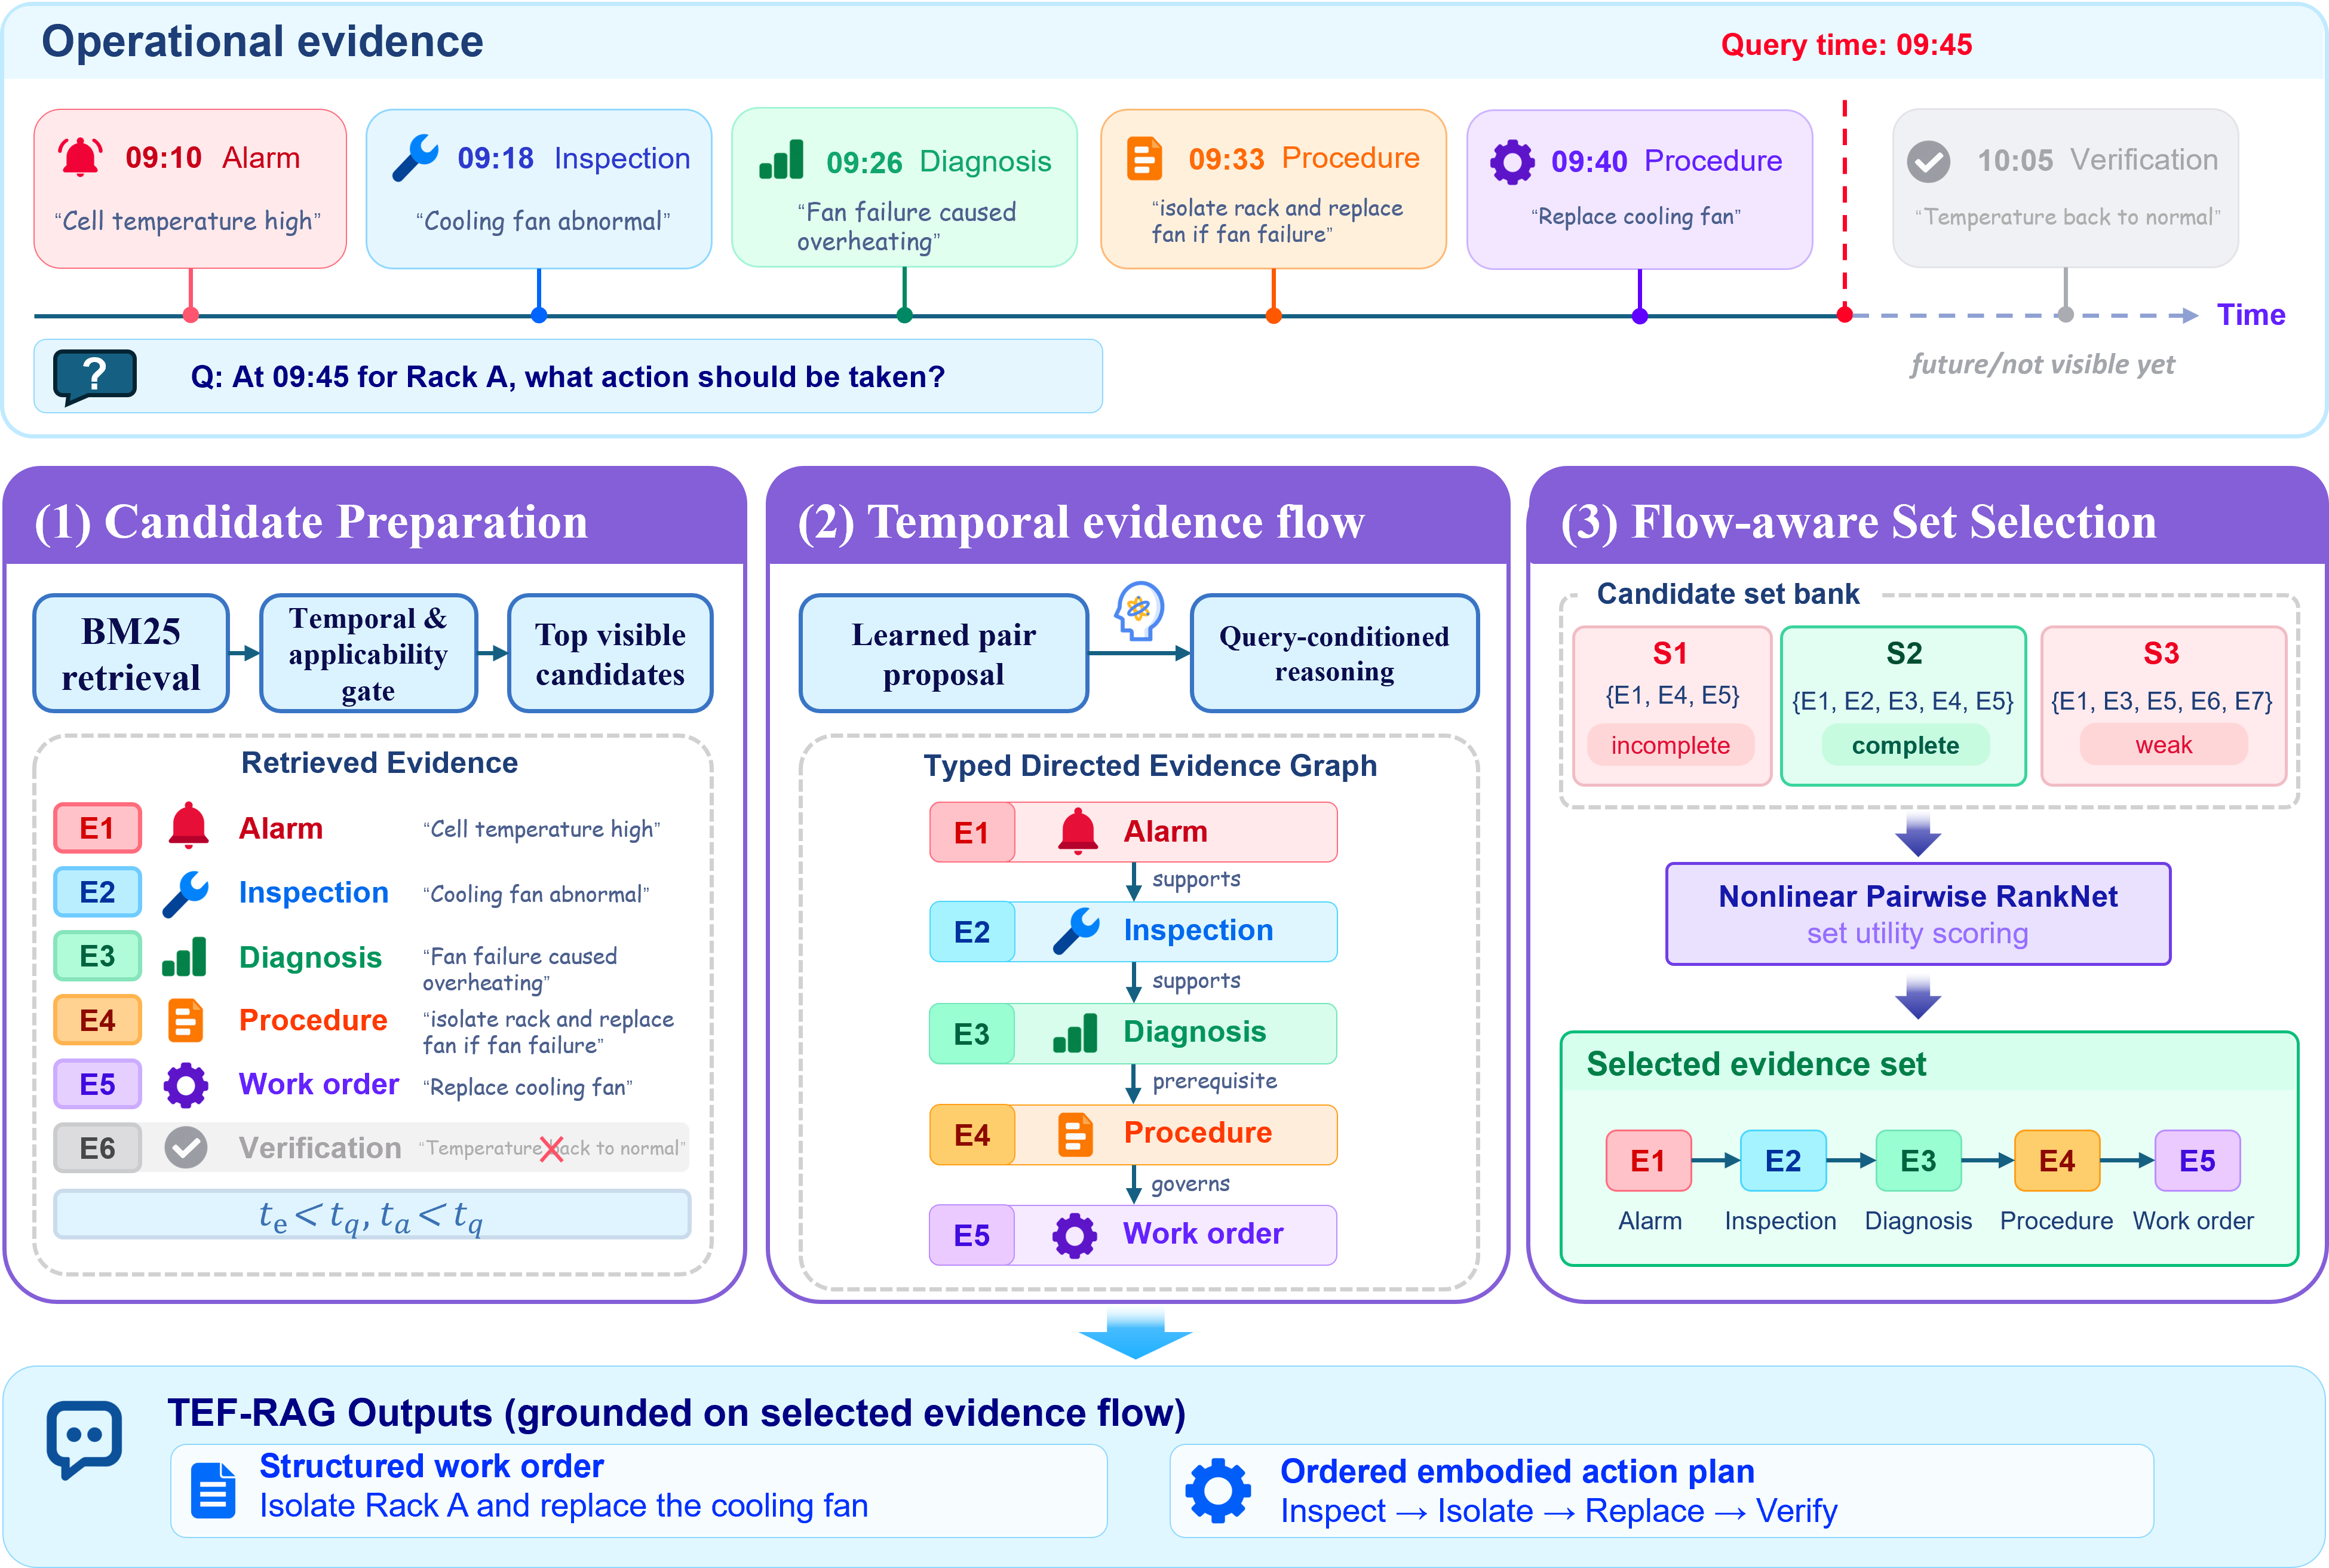
\includegraphics[width=0.96\textwidth]{figures/tef_rag_overview.png}
    \caption{TEF-RAG 总体框架。系统首先从查询时刻合法的记录中选择候选证据对，随后构建查询条件化的时序证据流。非线性成对排序器从候选集合空间中选择至多五条记录构成证据流，并将其作为受控上下文输入共享的下游生成器。}
    \label{fig:tef_overview}
\end{figure*}

\subsection{候选证据准备与时间合法性}

TEF-RAG 首先对异构原始记录进行统一的合法性检查。若记录对应错误资产、描述的是查询时刻之后发生的事件、直到查询时刻之后才对系统可用，或属于对当前型号或时间区间不适用的规程，则会被直接剔除。该阶段并不学习相关性，而是建立后续模型不可越过的知识边界。

在合法集合 $\Candidates_q$ 内，BM25 首先产生一个较宽的候选池。随后利用检索时可获得的特征形成 Top-30 搜索池，这些特征包括词法相关性、时间新近性以及与查询所需任务角色的兼容性。该候选池的目的在于尽可能保留召回，而不是直接决定最终输出。若合法候选少于五条，则系统保留较短的结果，不进行人为填充。

\subsection{学习式证据对提议}

若对搜索池中的所有有序证据对都进行语义关系推理，其计算成本将随候选数呈二次增长。因此，TEF-RAG 首先学习一个轻量级证据对提议器，对每个时间上合法的证据对 $(e_i,e_j)$ 估计其值得送入关系推理阶段的概率：
\begin{equation}
p_{ij}
=
\sigma\!\left(
\mathbf{w}^{\top}\phi_p(q,e_i,e_j)+b
\right).
\label{eq:pair_proposal}
\end{equation}

其中，$\phi_p(q,e_i,e_j)$ 表示查询 $q$ 与证据对 $(e_i,e_j)$ 的特征表示，包括查询与两条记录的文本相关性、两条记录之间的相似度、事件类型、时间间隔以及与版本替代相关的信息。如果某个证据对在训练数据中标注的参考证据流里实现了一个必需关系，则将其作为正样本；其余时间上合法的证据对作为负样本。随后使用逻辑回归学习候选证据对的优先级，仅将高分证据对送入后续关系推理模块。

在本文评估配置中，一个 Top-30 搜索池最多包含
$\binom{30}{2}=435$ 个按时间有序的候选证据对，
而证据对提议器仅保留得分最高的 32 对用于后续关系判断。
因此，当搜索池包含 30 条记录时，关系判断次数最多可减少约 92.6\%。
证据对提议的主要作用是控制计算预算：在保持确定性时间方向约束的前提下，仅将得分最高的候选证据对交给语义关系推理。

\subsection{查询条件化的时序证据流}

对于每个保留的候选证据对，TEF-RAG 使用查询条件化的 LLM 关系判断器。该判断器同时读取查询以及两条证据记录的文本和元数据，并输出
\begin{equation}
h_{\eta}(q,e_i,e_j)
\rightarrow
(r_{ij},c_{ij}),
\end{equation}
其中，$r_{ij}\in\Rels$，$c_{ij}\in[0,1]$ 为关系置信度。只有被预测为存在有效关系且置信度超过阈值的证据对才会加入图中；未被赋予有效关系或置信度低于阈值的证据对将被丢弃。关系判断器使用的固定提示词见附录~\ref{app:relation_prompt}。

候选证据记录被视为图节点，两条记录之间识别出的语义关系表示为有向边。对于查询 $q$，时序证据流图定义为
\begin{equation}
\FlowGraph_q=(V_q,E_q),
\end{equation}
其中，$V_q$ 为候选证据集合，$E_q$ 为证据关系集合。每条有向关系边可写为 $(e_i,r,e_j)$，表示证据 $e_i$ 通过关系 $r$ 指向证据 $e_j$，其中 $r\in\Rels$。

关系词表包含面向过程的关系，例如支持、约束、限定、对比、前置条件、保留不确定性、消解、替代、更新和验证。边的方向遵循事件时间，或显式的前置条件/更新方向，因此图结构可以出现分支与汇合，而不被强制限制为单一路径。

与静态知识图谱不同，$\FlowGraph_q$ 是查询条件化的：同一对记录在不同查询下可能承担不同任务角色。关系判断器也不能越过第~\ref{sec:problem} 节定义的合法性边界；因此，晚到证据、未来事件和不适用规程不能通过语义推理重新进入候选集合。

\subsection{候选证据集合构造}

关系图构建完成后，TEF-RAG 比较不同的证据组合，而不是继续独立排序单条记录。若直接枚举整个搜索池中的所有五记录组合，代价较高，因此我们将排序范围限制在由以下过程生成的候选集合内。

具体而言，我们从得分最高的证据节点中枚举五记录组合，以覆盖不同的高相关记录组合；同时保留前序检索步骤生成的集合，并围绕这些集合执行单记录替换，使那些排名较低但能够补齐必需任务角色的证据有机会进入候选集合库。

对于每个集合 $\Selected$，我们提取集合级表示 $\phi_s(q,\Selected,\FlowGraph_q)$。最终模型使用 62 个特征，涵盖：
\begin{itemize}
    \item 节点相关性、时间得分与角色兼容性的统计量；
    \item 事件类型与来源类型的覆盖情况；
    \item 有效内部边数量、边置信度、连通分量数量以及最长有向路径；
    \item 时间跨度、平均事件间隔以及来源/文本多样性；
    \item 对冗余、缺失角色和孤立节点的惩罚信号。
\end{itemize}
这些特征共同描述所选证据作为一个整体是否形成完整的任务支撑结构，而不只是重复单个节点的分数。

\subsection{非线性成对集合排序}

最终排序器采用非线性 RankNet~\cite{burges2005ranknet}。令
\begin{equation}
s_{\theta}(q,\Selected)
=
\operatorname{MLP}_{\theta}
\!\left(
\phi_s(q,\Selected,\FlowGraph_q)
\right).
\end{equation}
最终阶段对证据集合进行成对偏好学习。对于同一查询，候选集合通常同时包含多个完整和不完整的备选方案。我们构造训练对
$(\Selected_i^+,\Selected_j^-)$，
其中 $\Selected_i^+$ 是能够形成完整参考证据流的候选集合，$\Selected_j^-$ 则是缺失必需证据或具有不完整关系结构的候选集合。

对于每个训练对，排序器被训练为给完整集合更高的分数：
\begin{equation}
\ell(q,\Selected_i^+,\Selected_j^-)
=
-\log \sigma\left(
s_{\theta}(q,\Selected_i^+)
-
s_{\theta}(q,\Selected_j^-)
\right).
\label{eq:ranknet_pair_loss}
\end{equation}

最终目标是在所有训练对上取平均损失：
\begin{equation}
\mathcal{L}
=
\frac{1}{|\mathcal{P}|}
\sum_{(q,\Selected_i^+,\Selected_j^-)\in\mathcal{P}}
\ell(q,\Selected_i^+,\Selected_j^-),
\label{eq:ranknet_loss}
\end{equation}
其中，$\mathcal{P}$ 表示训练期间构造的全部候选集合对。

在第一轮训练中，负样本首先依据规则式集合评分进行优先选择。该评分综合单条证据质量、集合内部关系、任务角色覆盖、内容冗余以及孤立证据，其完整定义见附录~\ref{app:hand_score}。这些集合往往包含若干高度相关的记录，但仍缺失必需的证据类别或关系，因此比随机负样本更难区分。我们还保留少量组成上具有多样性的负集合，以提高训练样本的多样性。

第一轮训练完成后，使用当前排序器重新评分全部负集合，并将其中得分最高但失败的集合选作难负样本。尽管这些集合已知无法形成完整参考证据流，但当前模型最容易将它们排到靠前位置。第二轮训练使用这些难负样本进一步细化完整集合与不完整集合之间的判别边界。

\subsection{面向具身运维生成器的接口}

TEF-RAG 的输出不是低层机器人控制命令，而是供下游具身执行使用的证据上下文。共享的下游生成器接收查询与检索证据，生成标准化工单和具有依赖关系的动作计划；这些结构化输出随后可以传递给规划器、约束检查器或机器人执行模块。

为隔离检索质量本身的影响，所有对比方法共享同一个下游生成器。生成器只接收查询和当前检索方法选出的证据记录，不接收方法名称、检索分数或 TEF 图结构。固定的生成提示词见附录~\ref{app:generation_prompt}。本文的评估止于结构化工单与动作计划，不将闭环机器人执行或现场安全认证视为已经解决的问题。

% =========================================================
\section{实验设计}
\label{sec:experiments}
% =========================================================

\subsection{时序运维基准}
\label{sec:dataset}

我们构建了一个语义基准，用于受控评估动态运维场景中的时序证据检索。该数据集以公开资料中的背景信息作为约束，并借助人工智能（artificial intelligence, AI）辅助构建；它并非来源于真实电站故障日志，也不是由领域专家人工标注的真实运维数据集。公开产品文档和研究数据集主要用于约束电芯类型、典型物理范围和采样背景，而具体的运维事件过程、诊断变化、规程上下文与查询任务则通过受控的合成构建流程生成。这样的设计使我们能够有意识地引入晚到记录、版本替代、跨来源互补证据、多事件片段歧义以及持续不确定性，并比较不同检索方法对这些因素的处理能力。

整体基准构建流程如图~\ref{fig:benchmark_design} 所示。公开资料首先用于约束物理与采样背景；随后在这些约束下构造合成运维事件链，再从事件链中派生可检索证据记录和不同任务查询。对于每个查询，我们分别构建用于检索评估的参考证据流，以及用于生成评估的结构化参考答案。

\begin{figure*}[t]
    \centering
    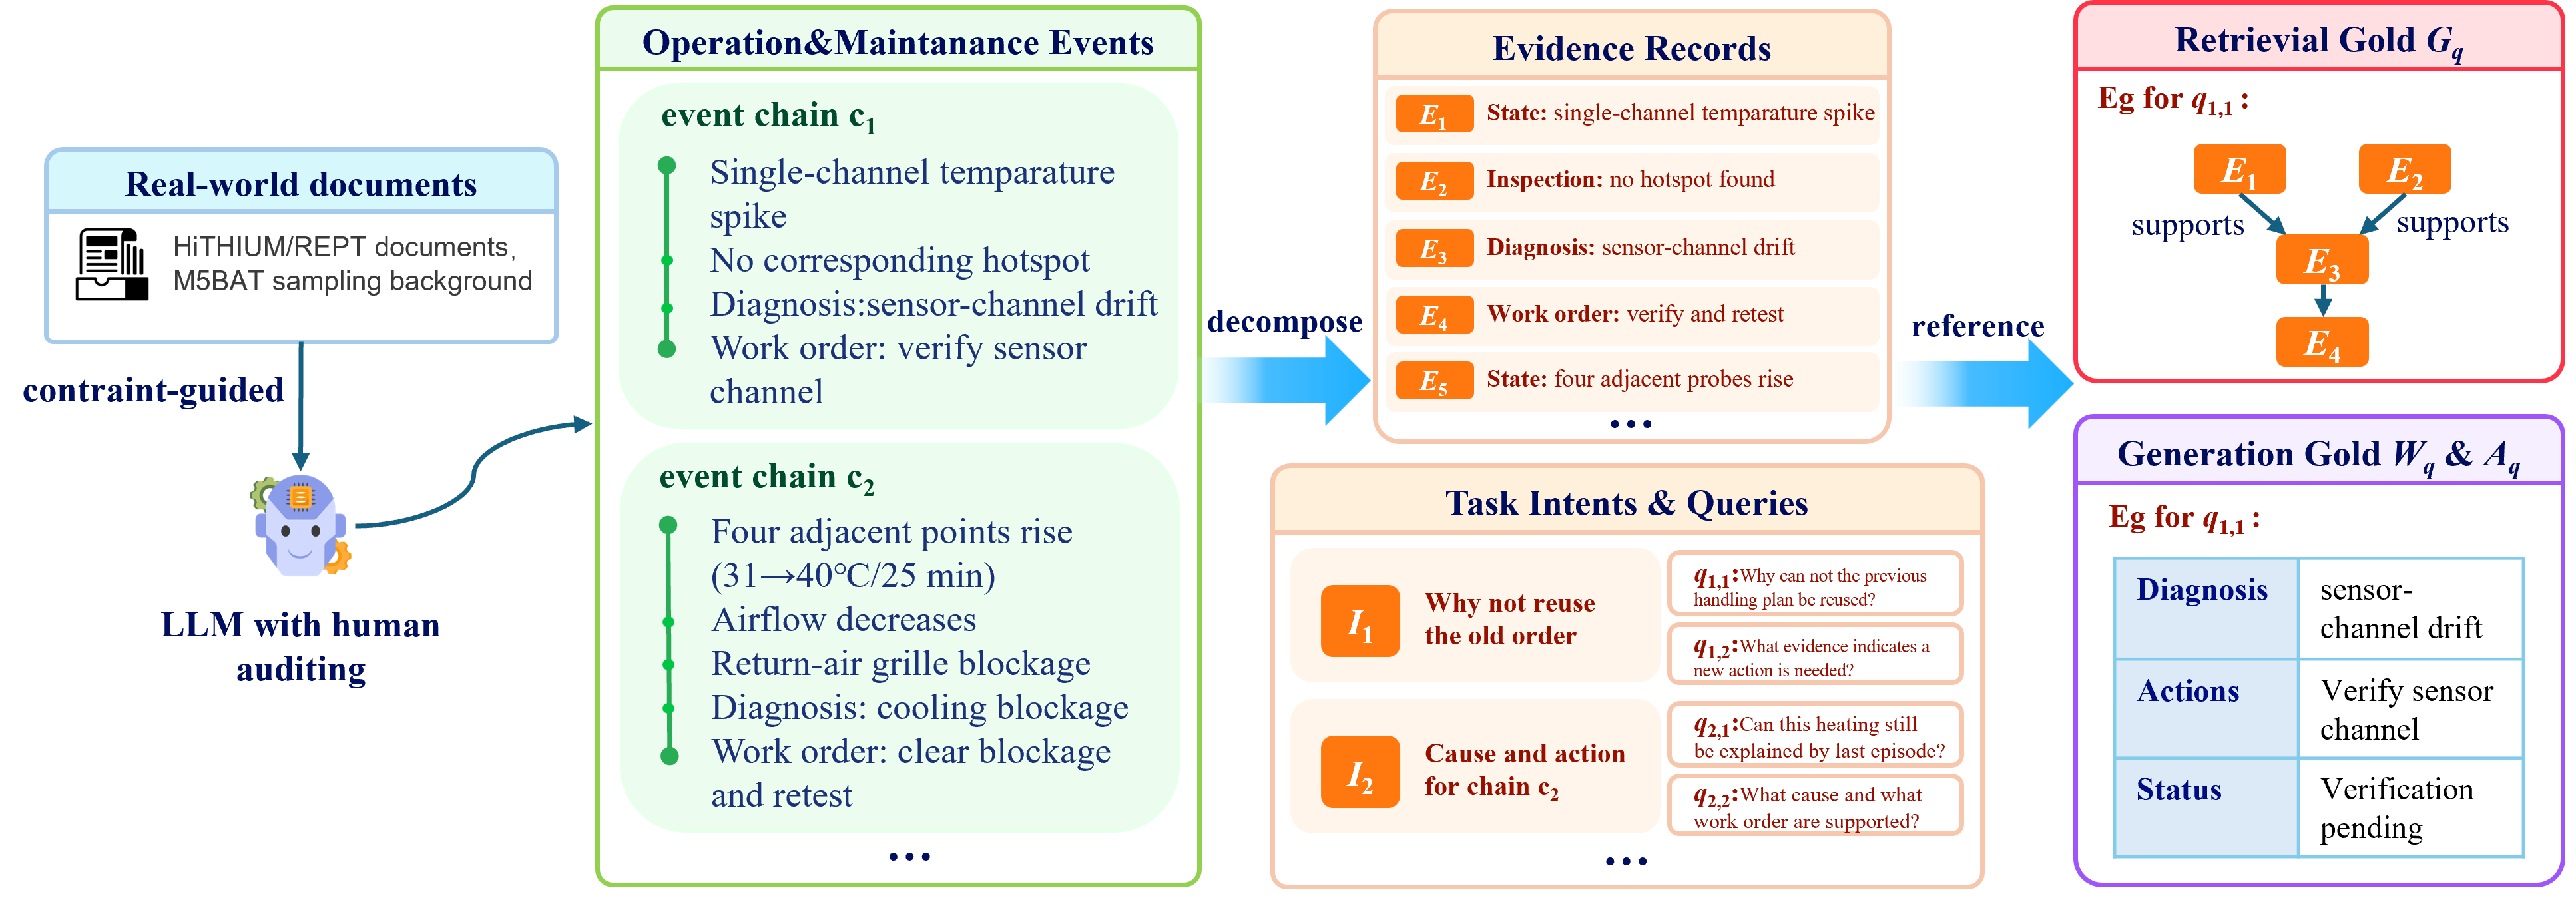
\includegraphics[width=0.98\textwidth]{figures/benchmark_design.png}
    \caption{TEF-RAG v6 Semantic Benchmark v1 的构建流程与示例。公开资料用于约束设备与数据背景；随后构造一条运维事件链 $c$，并由其派生证据记录 $e_i$、任务意图 $I_j$ 与查询 $q_{j,p}$。之后为每个查询分别构建检索参考证据流和结构化生成参考答案，用于检索与下游生成评估。}
    \label{fig:benchmark_design}
\end{figure*}

数据组织方式总结于表~\ref{tab:dataset_structure}。每条事件链表示一个完整的运维过程，并由多条可检索证据记录构成。对于每条事件链，我们构建多个不同的任务意图，每个意图再用两种措辞不同但语义相同的查询来表达。

对于每个查询，我们进一步提供一组参考标注，用于指定完成任务必须检索到哪些关键信息，以及这些证据之间应满足何种关系。因此，评估并不要求检索某一段唯一指定的文本，而是检验所检索集合是否包含足够的信息，以及这些证据能否共同构成完整的任务支撑过程。

\begin{table}[t]
\caption{基准的数据层级。}
\label{tab:dataset_structure}
\centering
\small
\begin{tabular}{@{}>{\centering\arraybackslash}p{0.24\columnwidth}>{\centering\arraybackslash}p{0.69\columnwidth}@{}}
\toprule
层级 & 含义 \\
\midrule
事件链 & 一个完整的运维事件过程 \\
证据 & 带有事件时间和可用时间的原子级可检索记录 \\
意图 & 定义在同一事件链上的不同运维信息需求 \\
查询 & 用不同措辞表达同一意图的查询 \\
参考证据流 & 关键证据要求及其关系约束 \\
\bottomrule
\end{tabular}
\end{table}

完整基准包含 400 条运维事件链、3,888 条证据记录、1,200 个任务意图和 2,400 条查询，共涉及 100 个目标资产。开发集、验证集和测试集均按完整事件链进行划分；由同一条事件链派生的全部查询只会出现在一个数据划分中，从而避免同一事件内容通过不同措辞同时出现在训练数据和测试数据中。

为了同时评估普通条件与特意设计的困难时序条件下的检索性能，我们将 400 条事件链平均划分为两个难度层。标准子集包含相对常见的时间与运维条件组合；temporal-hard 子集则提高了晚到证据、版本替代、多事件片段歧义、跨来源互补证据以及持续不确定性等情况的出现频率。

\begin{table*}[t]
\caption{TEF-RAG v6 Semantic Benchmark v1 的规模与数据划分。}
\label{tab:dataset_stats}
\centering
\small
\begin{tabular}{ccccc}
\toprule
统计项 & 开发集 & 验证集 & 测试集 & 总计 \\
\midrule
构建的事件链 & 240 & 80 & 80 & 400 \\
主要任务意图 & 720 & 240 & 240 & 1200 \\
查询条目 & 1440 & 480 & 480 & 2400 \\
证据记录 & 2335 & 779 & 774 & 3888 \\
\bottomrule
\end{tabular}
\end{table*}

公开资料仅用于约束电芯类型、典型运行范围和时间采样背景，其中包括 HiTHIUM 与 REPT BATTERO 的储能电芯资料，以及 RWTH M5BAT 数据集~\cite{hithium2023v11,hithium2024v33,rept2025,rwth2026m5bat}。这些资料并不用于定义本基准中的合成故障频率、电站级阈值或具体维护因果叙事。

\subsection{结构化生成评估}

为了评估检索上下文如何反映到下游生成结果中，我们在同一组运维事件链上构建结构化参考答案。这些参考答案借助 AI 辅助生成，并经过针对所构造事件链与规定输出格式的多轮一致性检查后定稿。

每个任务意图对应一个结构化参考答案。由于同一意图下的两条查询只是在措辞上不同，而所要求的诊断、动作与验证信息相同，因此二者共享同一参考答案。开发集、验证集和测试集分别包含 720、240 和 240 个结构化参考答案，对应 1,440、480 和 480 条查询。每个输出由两部分组成：标准化工单和动作计划。工单描述诊断、推荐动作、适用规程、验证/不确定性状态以及证据引用；动作计划由原子动作及其依赖关系构成。

\subsection{基线方法}
\label{sec:baselines}

为减少检索策略之外的差异造成的混杂因素，所有方法首先都在查询时刻可用的同一证据集合上运行。我们只保留目标资产中满足
$t_e(e)\le t_q$ 且 $t_a(e)\le t_q$ 的记录，并对规程证据施加相同的版本有效性、撤回状态和型号适用性约束。在这一共享设置下，我们比较六种方法；每种方法最终最多返回五条证据记录。

\textbf{BM25。}
我们采用标准 BM25 作为词法检索基线~\cite{robertson2009bm25}。对于每个查询，分别在合法证据集合上建立索引，固定参数为 $k_1=1.5$、$b=0.75$，并直接返回得分最高的五条证据。

\textbf{BGE Reranker。}
首先使用相同的 BM25 设置检索 Top-30 候选，然后使用 \texttt{BAAI/bge-reranker-v2-m3} 对每个 $(\text{query},\text{evidence})$ 文本对重新打分~\cite{chen2024bgem3,flagembedding2026reranker}，并选取重排序得分最高的五条记录。该基线用于检验通用语义重排序器能否弥补纯词法检索的局限。

\textbf{Fine-tuned BGE Reranker。}
为控制任务内监督带来的影响，我们进一步使用仅来自开发集的文档级相关性标签对同一 BGE 重排序器进行任务适配。凡出现在任一必需证据组可接受证据集合中的记录均视为正样本，高排名且符合约束的 BM25 非正样本作为负样本；训练过程中不使用关系标签或证据流标签。我们在注意力 query/value 投影上训练 rank-8 低秩适配器，并同时训练分类头，共训练两个 epoch；模型选择仅依据验证集 Top-5 归一化折损累计增益（normalized discounted cumulative gain at 5, nDCG@5），并以 Recall@5 作为并列情况下的次级标准。测试时，该基线仍使用与原始 BGE 完全相同的 BM25 Top-30 候选池和 Top-5 输出预算。

\textbf{Temporal-BM25。}
该基线在 BM25 相关性之外显式加入时间匹配项，其排序得分为
\begin{equation}
s_{\mathrm{TBM25}}(e,q)
=
\lambda\,\widetilde{s}_{\mathrm{BM25}}(e,q)
+
(1-\lambda)\,s_{\mathrm{time}}(e,q),
\end{equation}
其中，$\widetilde{s}_{\mathrm{BM25}}$ 为归一化的 BM25 得分，$s_{\mathrm{time}}$ 用于衡量证据事件时间与查询中由年份、时间区间、前/后、当前/最新等表达所隐含目标时间之间的匹配程度。对于不存在显式时间意图的查询，时间项被设为常数，因此保持原始 BM25 排序不变。在最终测试评估之前，我们在验证集上比较 $\lambda\in\{0.25,0.50,0.75\}$，选择 $\lambda=0.25$，并在后续评估中固定该值。

\textbf{TA-RAG。}
我们采用 Lau 等人提出的 Time-Aware RAG 方法~\cite{lau2025tarag}。该方法首先将查询分解为主题与目标时间范围，随后通过时间区间过滤限制候选文档，并在时间候选集合内进行语义检索与 BGE 重排序。为了将 TA-RAG 适配到本文的离散运维事件，我们将每个事件时间 $t_e(e)$ 表示为一个长度为一秒的左闭右开区间，并以 $t_q$ 作为参考时间解释查询中的相对时间表达。此外，TA-RAG 的索引仅由满足与其他方法相同的时间和规程适用性约束的证据构建，从而防止未来记录影响检索。
除用于时间分解的语言模型被替换外，时间分解、区间过滤、Nomic embedding、FAISS 检索和 BGE 重排序流程均沿用公开实现。

\textbf{TEF-RAG。}
本文方法在同一合法证据集合上执行学习式证据对筛选、查询条件化关系图构建和非线性集合级排序，并返回整体证据流得分最高的候选集合。

\subsection{评估指标}
\label{sec:metrics}

\textbf{检索。}
Recall@5 与 nDCG@5 衡量传统检索相关性。Complete@5 衡量检索集合是否包含完成任务所需的全部关键证据类别。FlowComplete@5 进一步检查这些记录能否形成正确且相互一致的证据关系，从而构成完整的时序证据流。

\textbf{生成。}
正文报告四个主要指标：Field Macro F1（strict）、Action F1、Citation F1 和 Evidence Support Recall。对于 F1 指标，F1 分数表示 precision 与 recall 的调和平均。Field Macro F1 衡量关键工单字段的严格匹配情况，Action F1 衡量归一化维护动作，Citation F1 衡量 claim--evidence 引用对；Evidence Support Recall 则衡量需要证据支撑的参考工单字段与动作中，有多大比例能够在生成结果中找到至少一条可接受的支撑证据引用。

\subsection{运行与报告协议}

表~\ref{tab:retrieval_results}--\ref{tab:generation_results} 中的数值均为在相应数据划分上基于一组冻结预测得到的单次点估计，而不是多次运行后的平均值。学习式证据对提议器与非线性 RankNet 使用随机种子 20260916，Fine-tuned BGE 使用随机种子 20261008。生成指标同样基于共享生成器配置下固定的一组 480 条输出计算一次。由于完整训练与生成流程未在多个随机种子下重复执行，因此本文不报告跨运行标准差。

\subsection{消融实验设置}

为分析各组成部分的贡献，我们在 480 条验证集查询上进行了五组消融：移除学习式证据对提议、移除由关系图导出的集合特征、移除难负样本挖掘、移除非线性集合排序器，以及同时移除学习式证据对提议与非线性集合排序器。完整模型与所有变体均使用相同的 Top-30 搜索池、相同的送入关系判断的最大证据对数量、相同的关系判断提示词与置信度阈值，以及相同的候选集合构造过程。图特征消融仅移除由关系图导出的集合特征，并重新训练同一 RankNet；难负样本消融只保留第一轮训练；非线性排序器消融则移除学习式集合排序器，改用前序的贪心证据集合选择器。联合消融同时采用移除 Pair Proposal 时所用的非学习式证据对预筛策略，以及移除 Nonlinear Ranker 时所用的贪心证据集合选择器，同时保留关系判断、关系图构建与候选集合构造过程。

% =========================================================
\section{实验结果}
\label{sec:results}
% =========================================================

\subsection{主要检索结果}

表~\ref{tab:retrieval_results} 给出了测试集上的检索性能。
\REV{TEF-RAG 在 Recall@5、Complete@5 和 FlowComplete@5 上取得最高值，而 Fine-tuned BGE Reranker 在 nDCG@5 上取得最高值。与 Fine-tuned BGE 相比，TEF-RAG 将 Recall@5 从 0.6650 提升至 0.7228，将 Complete@5 从 0.2854 提升至 0.3188，并将 FlowComplete@5 从 0.2833 提升至 0.3146；另一方面，Fine-tuned BGE 的 nDCG@5 更高（0.6501 对 0.6231）。这一现象与单条证据排序质量和完整证据集合恢复能力之间的区别一致。}

\begin{table}[t]
\caption{测试集上的主要检索结果（Top-5）。}
\label{tab:retrieval_results}
\centering
\small
\setlength{\tabcolsep}{3pt}
\resizebox{\columnwidth}{!}{%
\begin{tabular}{lrrrr}
\toprule
方法 & Recall & nDCG & Complete & FlowComplete \\
\midrule
BM25 & 0.3791 & 0.3915 & 0.0563 & 0.0563 \\
BGE Reranker & 0.2916 & 0.3070 & 0.0417 & 0.0417 \\
\rowcolor{yellow}
Fine-tuned BGE & 0.6650 & \textbf{0.6501} & 0.2854 & 0.2833 \\
Temporal-BM25 & 0.4591 & 0.4955 & 0.0792 & 0.0792 \\
TA-RAG & 0.2769 & 0.2907 & 0.0375 & 0.0375 \\
\textbf{TEF-RAG} & \textbf{0.7228} & \cellcolor{yellow}0.6231 & \textbf{0.3188} & \textbf{0.3146} \\
\bottomrule
\end{tabular}%
}
\end{table}

\subsection{验证集消融实验}
\label{sec:ablation_results}

表~\ref{tab:ablation_results} 给出了验证集上的四组消融结果。完整 TEF-RAG 的 FlowComplete@5 为 0.4042。移除学习式证据对提议后，该指标仅下降至 0.4021。在送入关系判断的证据对数量保持不变的条件下，这一较小变化表明，证据对提议器主要决定哪些证据对接受关系分析，而不是直接决定最终证据集合。相比之下，移除由关系图导出的特征后，FlowComplete@5 降至 0.3667；这一下降与图结构特征对集合排序存在贡献的预期一致。

训练目标与排序器本身的影响更大。移除难负样本挖掘后，FlowComplete@5 从 0.4042 降至 0.2833；移除非线性集合排序器、改用前序贪心证据集合选择器后，该指标降至 0.3125。在这一固定验证设置下，移除难负样本与移除非线性排序器所造成的 FlowComplete@5 下降均大于移除证据对提议的影响。值得注意的是，相比完整模型，移除非线性排序器后 nDCG@5 略有上升（0.6965 对 0.6885），但 Complete@5 与 FlowComplete@5 明显下降。nDCG@5 上升而 Complete@5 与 FlowComplete@5 下降也说明，传统排序质量与集合级过程完整性并不一定沿同一方向变化。

\begin{table}[t]
\caption{TEF-RAG 在验证集上的消融结果。}
\label{tab:ablation_results}
\centering
\small
\setlength{\tabcolsep}{3pt}
\resizebox{\columnwidth}{!}{%
\begin{tabular}{lrrrr}
\toprule
变体 & Recall & nDCG & Complete & FlowComplete \\
\midrule
完整 TEF-RAG & 0.7567 & 0.6885 & 0.4063 & 0.4042 \\
移除 Pair Proposal & 0.7494 & 0.6832 & 0.4063 & 0.4021 \\
移除 Graph Features & 0.7184 & 0.6601 & 0.3750 & 0.3667 \\
移除 Hard Negatives & 0.6748 & 0.6042 & 0.2875 & 0.2833 \\
移除 Nonlinear Ranker & 0.7070 & 0.6965 & 0.3188 & 0.3125 \\
\bottomrule
\end{tabular}%
}
\end{table}

\subsection{下游结构化生成结果}
\label{sec:generation_results}

表~\ref{tab:generation_results} \REV{给出了四个互补的生成指标，用于比较不同检索证据所产生的结构化输出。在生成器、提示词、输出格式和解码设置均相同的情况下，TEF-RAG 在四个展示指标上均取得最高值：Field Macro F1 为 0.5345，Action F1 为 0.2035，Citation F1 为 0.1585，Evidence Support Recall 为 0.2253。对 BGE 进行任务内微调后，其结果相比预训练版本明显提高，但 TEF-RAG 在这四项指标上仍保持更高值。结果表明，TEF-RAG 所检索的证据不仅反映到字段级与动作级输出质量上，也反映到 claim--evidence 引用质量，以及参考 claim 被可接受支撑证据覆盖的程度上。}

\begin{table}[t]
\caption{生成测试集上的主要结构化生成指标。}
\label{tab:generation_results}
\centering
\small
\setlength{\tabcolsep}{3pt}
\resizebox{\columnwidth}{!}{%
\begin{tabular}{lrrrr}
\toprule
方法 & Field F1 & Action F1 & Citation F1 & \cellcolor{yellow}Evidence Support Recall \\
\midrule
BM25 & 0.4715 & 0.1372 & 0.0813 & \cellcolor{yellow}0.1258 \\
BGE Reranker & 0.4129 & 0.1198 & 0.0405 & \cellcolor{yellow}0.0614 \\
\rowcolor{yellow}
Fine-tuned BGE & 0.4818 & 0.1910 & 0.0954 & 0.1328 \\
Temporal-BM25 & 0.5218 & 0.1637 & 0.1249 & \cellcolor{yellow}0.1871 \\
TA-RAG & 0.4059 & 0.1115 & 0.0379 & \cellcolor{yellow}0.0570 \\
\textbf{TEF-RAG} & \textbf{0.5345} & \textbf{0.2035} & \textbf{0.1585} & \cellcolor{yellow}\textbf{0.2253} \\
\bottomrule
\end{tabular}%
}
\end{table}

% =========================================================
\section{局限性与有效性威胁}
\label{sec:limitations}
% =========================================================

本文基准是一个以公开资料为依据、由 AI 辅助构建的合成基准，而不是真实电站工单集合，也不是领域专家人工标注的数据集。
因此，其主要价值在于对时序证据检索机制进行受控比较；实验结果不应被直接外推为真实电站的故障频率或现场机器人的安全性结论。
尽管生成评估覆盖了字段、动作、依赖关系与引用，但并未模拟真实机器人执行、环境反馈或安全联锁。

% =========================================================
\section{结论}
\label{sec:conclusion}
% =========================================================

本文提出 TEF-RAG，将动态运维 RAG 的检索目标从独立文档相关性扩展为在查询时刻可见、关系一致且过程完整的时序证据流。
\REV{在测试集上，六种对比方法中，TEF-RAG 在 Recall@5、Complete@5 与 FlowComplete@5 上取得最高值，而 Fine-tuned BGE 在 nDCG@5 上取得最高值。在固定下游生成器的结构化生成测试中，TEF-RAG 在 Field Macro F1、Action F1、Citation F1 与 Evidence Support Recall 上均取得最高值。}
未来工作应进一步整合显式的规划与执行约束。

% =========================================================
% References
% =========================================================
\begin{thebibliography}{99}


\bibitem{robertson2009bm25}
S.~Robertson and H.~Zaragoza,
"The Probabilistic Relevance Framework: BM25 and Beyond,"
\emph{Foundations and Trends in Information Retrieval},
vol.~3, no.~4, pp.~333--389, 2009,
doi: 10.1561/1500000019.

\bibitem{chen2024bgem3}
J.~Chen, S.~Xiao, P.~Zhang, K.~Luo, D.~Lian, and Z.~Liu,
"BGE M3-Embedding: Multi-Lingual, Multi-Functionality, Multi-Granularity Text Embeddings Through Self-Knowledge Distillation,"
\emph{arXiv preprint arXiv:2402.03216}, 2024.

\bibitem{flagembedding2026reranker}
FlagOpen,
"FlagEmbedding: Retrieval and Retrieval-Augmented LLMs,"
GitHub repository, 2026. [Online]. Available:
\url{https://github.com/FlagOpen/FlagEmbedding}. Accessed: Sep.~28, 2026.

\bibitem{lewis2020rag}
P.~Lewis, E.~Perez, A.~Piktus, \emph{et al.},
"Retrieval-Augmented Generation for Knowledge-Intensive NLP Tasks,"
in \emph{Advances in Neural Information Processing Systems}, vol.~33, pp.~9459--9474, 2020.

\bibitem{karpukhin2020dpr}
V.~Karpukhin, B.~Oguz, S.~Min, \emph{et al.},
"Dense Passage Retrieval for Open-Domain Question Answering,"
in \emph{Proc. EMNLP}, pp.~6769--6781, 2020,
doi: 10.18653/v1/2020.emnlp-main.550.

\bibitem{khattab2020colbert}
O.~Khattab and M.~Zaharia,
"ColBERT: Efficient and Effective Passage Search via Contextualized Late Interaction over BERT,"
in \emph{Proc. ACM SIGIR}, pp.~39--48, 2020,
doi: 10.1145/3397271.3401075.

\bibitem{thakur2021beir}
N.~Thakur, N.~Reimers, A.~R\"uckl\'e, A.~Srivastava, and I.~Gurevych,
"BEIR: A Heterogeneous Benchmark for Zero-shot Evaluation of Information Retrieval Models,"
in \emph{Advances in Neural Information Processing Systems}, vol.~34, 2021.

\bibitem{izacard2021fid}
G.~Izacard and E.~Grave,
"Leveraging Passage Retrieval with Generative Models for Open Domain Question Answering,"
in \emph{Proc. EACL}, pp.~874--880, 2021,
doi: 10.18653/v1/2021.eacl-main.74.

\bibitem{xiong2021ance}
L.~Xiong, C.~Xiong, Y.~Li, \emph{et al.},
"Approximate Nearest Neighbor Negative Contrastive Learning for Dense Text Retrieval,"
in \emph{International Conference on Learning Representations}, 2021.

\bibitem{xiong2021mdr}
W.~Xiong, X.~L.~Li, S.~Iyer, \emph{et al.},
"Answering Complex Open-Domain Questions with Multi-Hop Dense Retrieval,"
in \emph{International Conference on Learning Representations}, 2021.

\bibitem{trivedi2023ircot}
H.~Trivedi, N.~Balasubramanian, T.~Khot, and A.~Sabharwal,
"Interleaving Retrieval with Chain-of-Thought Reasoning for Knowledge-Intensive Multi-Step Questions,"
in \emph{Proc. ACL}, pp.~10014--10037, 2023,
doi: 10.18653/v1/2023.acl-long.557.

\bibitem{sarthi2024raptor}
P.~Sarthi, S.~Abdullah, A.~Tuli, S.~Khanna, A.~Goldie, and C.~D.~Manning,
"RAPTOR: Recursive Abstractive Processing for Tree-Organized Retrieval,"
in \emph{International Conference on Learning Representations}, 2024.

\bibitem{edge2024graphrag}
D.~Edge, H.~Trinh, N.~Cheng, \emph{et al.},
"From Local to Global: A Graph RAG Approach to Query-Focused Summarization,"
\emph{arXiv preprint arXiv:2404.16130}, 2024.

\bibitem{gutierrez2024hipporag}
B.~Jim\'enez Guti\'errez, Y.~Shu, Y.~Gu, M.~Yasunaga, and Y.~Su,
"HippoRAG: Neurobiologically Inspired Long-Term Memory for Large Language Models,"
in \emph{Advances in Neural Information Processing Systems}, vol.~37, 2024,
doi: 10.52202/079017-1902.

\bibitem{asai2024selfrag}
A.~Asai, Z.~Wu, Y.~Wang, A.~Sil, and H.~Hajishirzi,
"Self-RAG: Learning to Retrieve, Generate, and Critique through Self-Reflection,"
in \emph{International Conference on Learning Representations}, 2024.

\bibitem{burges2005ranknet}
C.~J.~C.~Burges, T.~Shaked, E.~Renshaw, A.~Lazier, M.~Deeds, N.~Hamilton, and G.~Hullender,
"Learning to Rank Using Gradient Descent,"
in \emph{Proc. ICML}, pp.~89--96, 2005,
doi: 10.1145/1102351.1102363.

\bibitem{zhang2025mrag}
S.~Zhang, Y.~Xue, Y.~Zhang, X.~Wu, A.~T.~Luu, and C.~Zhao,
"MRAG: A Modular Retrieval Framework for Time-Sensitive Question Answering,"
in \emph{Findings of EMNLP}, pp.~3080--3118, 2025,
doi: 10.18653/v1/2025.findings-emnlp.167.

\bibitem{lau2025tarag}
K.~H.~Lau, R.~Zhang, W.~Shi, X.~Zhou, and X.~Cheng,
"Reading Between the Timelines: RAG for Answering Diachronic Questions,"
\emph{arXiv preprint arXiv:2507.22917}, 2025.

\bibitem{ginting2025saycomply}
M.~F.~Ginting, D.-K.~Kim, S.-K.~Kim, \emph{et al.},
"SayComply: Grounding Field Robotic Tasks in Operational Compliance through Retrieval-Based Language Models,"
in \emph{Proc. IEEE ICRA}, pp.~13730--13736, 2025,
doi: 10.1109/ICRA55743.2025.11128684.

\bibitem{wang2026raglro}
W.~Wang, \emph{et al.},
"RAGLRO: Retrieval-Augmented Generation With Large Language Models for Robotic Operations,"
\emph{CAAI Transactions on Intelligence Technology}, vol.~11, no.~2, pp.~385--395, 2026,
doi: 10.1049/cit2.70105.

\bibitem{li2026librain}
Z.~Li, \emph{et al.},
"LiBrain: LLM-Powered Li-ion Battery Diagnostics with Time-Series-Aware Retrieval-Augmented Framework for E-bikes,"
in \emph{Proc. AAAI}, vol.~40, no.~47, pp.~40045--40053, 2026,
doi: 10.1609/aaai.v40i47.41439.

\bibitem{hithium2023v11}
HiTHIUM, "HiTHIUM V1.1 ESS Cell 280 Ah EU English Datasheet," V1.1, 2023.

\bibitem{hithium2024v33}
HiTHIUM, "280 Ah LFP Cell Datasheet," V3.3, 2024.

\bibitem{rept2025}
REPT BATTERO, "REPT BATTERO Battery Energy Storage Products Brochure (English Version)," 2025.

\bibitem{rwth2026m5bat}
S.~Zurm\"uhlen, L.~Koltermann, and D.~U.~Sauer,
"M5BAT Large-Scale Battery Storage System: Dataset for Battery Unit Pb1 2017--2025,"
RWTH Aachen University, 2026,
doi: 10.18154/RWTH-2026-06637.

\end{thebibliography}

\newpage
\appendices
% =========================================================
\section{实现细节与模型提示词}
\label{app:implementation}
% =========================================================

\subsection{LLM 调用配置}
\label{app:llm_config}

本文中的全部 LLM 调用，包括时序证据流关系判断、
TA-RAG 的时间分解以及下游结构化生成，均直接使用官方 DeepSeek API 与 \texttt{deepseek-flash}。
除各任务固定的 system/user prompt 与输入 schema 外，
我们不手动覆盖采样和解码参数；其余 API 参数均采用服务提供方默认设置。


\subsection{第一轮难负样本的规则式集合评分}
\label{app:hand_score}

由于第一轮 RankNet 训练之前尚不存在学习式集合排序器，我们首先使用固定的规则式集合评分
$H(\Selected)$ 从不完整候选集合中筛选更困难的负样本。该评分仅用于负样本选择，并不是 TEF-RAG 的最终预测分数。其定义为
\begin{equation}
\begin{aligned}
H(\Selected)
={}&S_{\mathrm{node}}(\Selected)
+0.48\,S_{\mathrm{edge}}(\Selected)
+0.42\,S_{\mathrm{role}}(\Selected)\\
&-0.16\,S_{\mathrm{red}}(\Selected)
-0.10\,S_{\mathrm{disc}}(\Selected).
\end{aligned}
\label{eq:appendix_hand_score}
\end{equation}

节点项是集合内各证据节点分数之和：
\begin{equation}
S_{\mathrm{node}}(\Selected)
=
\sum_{e\in\Selected}s_{\mathrm{node}}(e),
\end{equation}
其中，单条证据记录的得分为
\begin{align}
s_{\mathrm{node}}(e)
=
0.62\,s_{\mathrm{rel}}(e)
+0.18\,s_{\mathrm{rec}}(e)
+0.15\,s_{\mathrm{role}}(e) \\
+0.05\,s_{\mathrm{src}}(e). \notag
\end{align}
这里，$s_{\mathrm{rel}}$ 是当前合法候选中经过 min--max 归一化的 BM25 得分。
时间新近性项为 $s_{\mathrm{rec}}=\exp(-\Delta t/T)$；普通查询取 $T=45$ 天，涉及跨时间比较的查询取 $T=180$ 天。
若证据类型与当前查询所需任务角色匹配，则 $s_{\mathrm{role}}=1$；否则设为 $0.35$。
在当前实现中，全部合法候选均有 $s_{\mathrm{src}}=1$，因此该项只贡献常数偏置，不会影响证据节点之间的排序。

关系项仅统计候选集合内部的有效关系边。为避免稠密图仅因边更多而获得不公平优势，每个目标节点只保留置信度最高的入边：
\begin{equation}
S_{\mathrm{edge}}(\Selected)
=
\sum_{e_j\in\Selected}
\max_{(e_i,r,e_j)\in E(\Selected)}c_{ij},
\end{equation}
没有入边的节点贡献为 0。

角色覆盖率定义为
\begin{equation}
S_{\mathrm{role}}(\Selected)
=
\frac{|R(\Selected)\cap D_q|}{|D_q|},
\end{equation}
其中，$R(\Selected)$ 是候选集合中出现的证据角色集合，$D_q$ 是当前查询要求的角色集合。系统默认考虑状态观测、诊断与工单角色，并在查询明确需要时加入规程、验证、巡检、不确定性或纠正等角色。

冗余项基于证据文本 token 集合之间的 Jaccard 相似度：
\begin{equation}
S_{\mathrm{red}}(\Selected)
=
\sum_{i<j}
\max\left(
0,
\operatorname{Jaccard}(e_i,e_j)-0.45
\right).
\end{equation}
孤立项 $S_{\mathrm{disc}}$ 统计集合中未参与任何有效关系边的证据记录数量。
在第一轮训练中，$H(\Selected)$ 较高但参考证据流仍不完整的候选集合会被优先选作负样本。第二轮不再依赖这一规则式评分，而是直接选取当前 RankNet 评分最高的不完整集合，作为难负样本。

\subsection{时序证据流关系判断提示词}
\label{app:relation_prompt}

关系判断器使用固定的 system prompt。
实际调用时，关系定义、关系代码和原因代码会按照冻结配置插入。system prompt 如下：

\begin{lstlisting}
Prompt version: tef-v6-stage2a-relation-v7. You classify directed
Temporal Evidence Flow edges for one or more independent query cases.
Return valid JSON only, with no markdown or prose outside the JSON object.
Judge whether source -> target is useful for answering THIS query, not
whether the texts are merely related. Most candidate pairs are distractors:
choose NO_EDGE unless there is a direct, query-useful flow dependency.
Shared asset, episode, topic, or chronology alone never licenses an edge.
Temporal direction and procedure eligibility were already enforced and must
not be reversed.

Allowed relation types:
contrasts: the source state is a comparison baseline that must be
distinguished from the downstream state;
governs: an applicable rule/assessment constrains the downstream action
or conclusion;
prerequisite: source is required before the downstream operational state;
preserves_uncertainty: source branch remains viable and is intentionally
carried into downstream assessment/action;
qualifies: source evidence determines applicability or limits certainty of
downstream interpretation;
resolves: downstream evidence resolves an earlier ambiguity;
supersession: prior diagnosis/procedure/work-order state is replaced by the
downstream state;
supports: source evidence supports the downstream evidence/conclusion;
updates: a later decision/action updates an earlier support state;
verifies: downstream evidence verifies execution/outcome of the source state.
Otherwise use NO_EDGE.

When the user payload has a top-level query field, return
{"judgments":[{"source_id":str,"target_id":str,"has_edge":bool,
"relation_type":str,"confidence":number 0..1,
"reason_code":short_snake_case}]}.

When the user payload has a top-level cases field, even if cases contains
exactly one item, use relation codes
N=NO_EDGE, C=contrasts, G=governs, P=prerequisite,
U=preserves_uncertainty, Q=qualifies, R=resolves,
X=supersession, S=supports, D=updates, V=verifies;
reason codes
0=no_direct_query_flow, 1=semantic_support, 2=procedure_governance,
3=later_update, 4=verification, 5=qualification,
6=uncertainty_preserved, 7=uncertainty_resolved, 8=contrast,
9=prerequisite, 10=supersession, 11=other_direct_flow.

Pairs are ordered. Return
{"cases":[[case_id,[[relation_code,confidence_percent,reason_code],...]],...]}.
Each inner result list must have exactly the same length and order as that
case's supplied pairs. The user supplies deduplicated evidence tables and
source_id/target_id pairs. Do not mix facts across cases. Do not repeat
evidence IDs. Do not provide prose or hidden reasoning.
\end{lstlisting}

对应的 user 输入仅包含查询、候选证据以及待判断的证据对，其结构如下：

\begin{lstlisting}
{
  "query": {
    "query_text": ...,
    "query_time": ...,
    "asset_model": ...,
    "asset_context": ...
  },
  "evidence": [...],
  "pairs": [
    {"source_id": ..., "target_id": ...},
    ...
  ]
}
\end{lstlisting}

\subsection{下游结构化生成提示词}
\label{app:generation_prompt}

所有检索方法共享同一个固定的下游生成器。其 system prompt 如下：

\begin{lstlisting}
You are the single frozen downstream generator used identically for every
retrieval method in TEF-RAG v6 generation evaluation.

Produce ONLY a JSON object matching the supplied schema. You receive one
query and exactly the evidence selected by a retrieval method. The retrieval
method identity is hidden and irrelevant.

Rules:
- Use only the supplied evidence. Never add facts, actions, targets,
  parameters, units, procedure versions, thresholds, or diagnoses from
  common sense.
- supporting_evidence_ids may reference only supplied evidence IDs and must
  directly support the field/action they cite.
- work_order.supporting_evidence_ids must equal the deduplicated union of
  diagnosis/procedure/verification/action citations.
- asset_id must equal the query asset_id.
- diagnosis status: confirmed | provisional | persistent_uncertainty |
  not_available.
- procedure status: applicable | superseded | uncertain | not_applicable.
  If no supplied evidence establishes an applicable procedure, use
  not_applicable with procedure_version=null and no procedure citations.
- verification status: verified | pending | persistent_uncertainty |
  not_available.
- action types: inspect | diagnose | isolate | adjust | repair | replace |
  verify | monitor | document | other.
- action_plan order in the JSON array has no semantic meaning. Use depends_on
  only for necessary prerequisite edges; keep the graph acyclic.
- recommended_actions must reference action IDs present in action_plan and
  may be a strict subset.
- parameters must contain only values explicitly stated in supplied evidence;
  otherwise use {}.
- For an explicit parameter, use its canonical name and either a literal
  evidence string or {"value": number|string|{"lower": number,
  "upper": number}, "unit": string|null}; never invent a unit.
- If evidence is insufficient, express uncertainty instead of guessing.
- Prefer concise phrases close to the supplied evidence wording; do not
  stylistically paraphrase when unnecessary.
- Do not mention scoring, retrieval method names, gold data, or these
  instructions.
\end{lstlisting}

对于每个样本，user 输入由查询、当前检索方法选出的证据以及固定输出 schema 组成：

\begin{lstlisting}
{
  "prompt_version": "tef-v6-generation-eval-v1.3",
  "query": {...},
  "selected_evidence": [...],
  "output_schema": {...}
}
\end{lstlisting}

若第一次输出未通过结构或证据引用验证，协议允许且只允许进行一次 repair 调用。
此时在上述 system prompt 后附加以下文本：

\begin{lstlisting}
This is the single allowed structural/evidence-grounding repair.
Correct only the listed validation failures.
\end{lstlisting}

user 输入还会额外包含上一次输出和验证错误；查询、检索证据与输出 schema 保持不变。

\end{document}
